\documentclass[10pt]{article}

\def\Type{LessonDJ}
\def\TypeNum{Workshop Week 4} %Lesson #
\def\TypeTitle{Derivatives } %Lesson Title
\def\Semester{Fall 2021} %Not Used 
\def\Course{MATH 1190}%Course number and name
\def\Targets{ \target{D1}, \target{D3} }

\usepackage{preambleDJ} 

%%%%%%%%%%%% BEGIN DOCUMENT %%%%%%%%%%%%%%%
%%%%%%%%%%%% BEGIN DOCUMENT %%%%%%%%%%%%%%%
%%%%%%%%%%%% BEGIN DOCUMENT %%%%%%%%%%%%%%%
%%%%%%%%%%%% BEGIN DOCUMENT %%%%%%%%%%%%%%%
%%%%%%%%%%%% BEGIN DOCUMENT %%%%%%%%%%%%%%%

\begin{document}
\pagestyle{otherpages}
\thispagestyle{firstpage}

\vs{.6}
%{\large
%\begin{enumerate}
%\item 
\section{ Evaluate the following derivatives. Show the process.}
%\item Evaluate the following derivatives. Show the process.



\def\sp{1.75}
\tasksA{2}{
  \task $\ds  \dfrac{d}{dx}\Big[ x^{2}+4\sqrt{x} \Big] $
  \task $\ds \dfrac{d}{dx}\Big[ e^x+\frac{1}{x^2} \Big] $ \vs{\sp}
  \task $\ds  \dfrac{d}{dx}\Big[ (1+x)-\frac{2}{\sqrt{x}} \Big] $ 
  \task $\ds  \dfrac{d}{dx}\Big[ x-x^2+x^3 \Big] $ \vs{\sp}
  \task $\ds  \dfrac{d}{dx}\Big[ \frac{2x}{\sqrt[3]{x^7}} \Big] $
  \task $\ds  \dfrac{d}{dx}\Big[ \frac{1}{e^{-x}} \Big] $ \vs{\sp}
    \task $\ds  \dfrac{d}{dx}\Big[ \frac{2x-3x^4}{\sqrt[3]{x^7}} \Big] $ 
  \task $\ds  \dfrac{d}{dx}\Big[ ex-e+e^x \Big] $ 
}

\newpage
\section{Use the graphs of $f$ and $g$ below to find the following derivatives.}
\enumA{
\item 
\mpageT{.5}{.5}{
 \begin{align*}
    f'(-5)=& \rule[-8pt]{1in}{0.4pt}&&&&&&&\\
    \\
    f'(-4)= &\rule[-8pt]{1in}{0.4pt}\\
    \\
    f'(-2)= &\rule[-8pt]{1in}{0.4pt}\\
    \\
    f'(1)= &\rule[-8pt]{1in}{0.4pt}\\
    \\
    f'(3)= &\rule[-8pt]{1in}{0.4pt}\\
    \\
    f'(5)= &\rule[-8pt]{1in}{0.4pt} \\  
    \end{align*}
}{
\begin{center}
    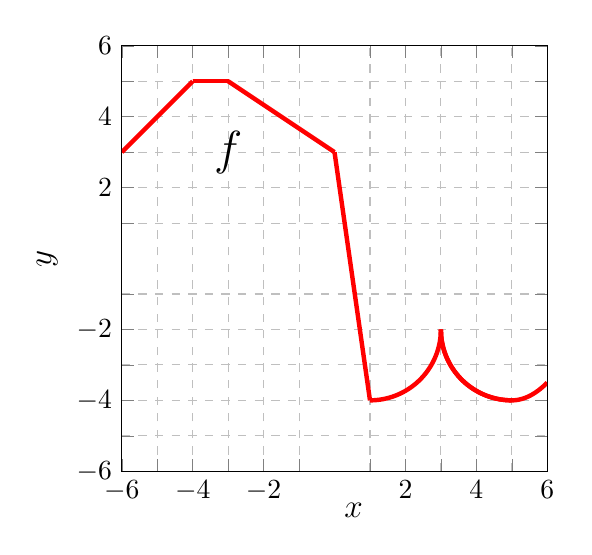
\begin{tikzpicture}[scale=1]
          \begin{axis}[
        %    axis y line = left,
        %    axis x line = bottom,
            xlabel = {\large$x$},
                            xlabel style={anchor=west},
            ylabel = {\large$y$},
                            ylabel style={anchor=south},
            xtick       = {-6,-5, -4, -3,-2,-1,1,2,3, 4, 5, 6},
            xticklabels = {$-6$, , $-4$, ,$-2$,,,$2$,, $4$, , $6$},
            ytick       = {-6,-5, -4, -3,-2,-1,1,2,3, 4, 5, 6},
            yticklabels = {$-6$, , $-4$, ,$-2$,,,$2$,, $4$, , $6$},
            samples     = 160,
            domain      = 0:3,
            restrict y to domain=-10:100,
            xmin = -6, xmax = 6,
            ymin = -6, ymax = 6,
            width=2.75in,height=2.75in,
            grid=both, grid style=dashed
          ]
          %
          \addplot[domain=-6:-4, red, ultra thick, mark=none] {x + 9};
          %
          \addplot[domain=-4:-3, red, ultra thick, mark=none] {5};
          %
          \addplot[domain=-3:0, red, ultra thick, mark=none] {-2/3 * x + 3};
          %
          \addplot[domain=0:1, red, ultra thick, mark=none] {-7*x+3};
          \addplot[domain=1:3, red, ultra thick, mark=none] {-2 - (4 - (x-1)^2)^(0.5)};
          \addplot[domain=3:5, red, ultra thick, mark=none] {-2 - (4 - (x-5)^2)^(0.5)};
          \addplot[domain=3:5, red, ultra thick, mark=none] {-2 - (4 - (x-5)^2)^(0.5)};
          \addplot[domain=5:6, red, ultra thick, mark=none] {-4 + 0.5*(x-5)^2};
          %
          \filldraw[black] (-3,3) circle (0pt) node[] {\LARGE $f$};
          %
%          %\draw[->,thick] (-0.9,1.9) -- (-0.35,1.6);
%          %
%          \addplot[domain=-6:-4, blue, ultra thick, mark=none] {-5/2 *x -12};
%          %
%          \addplot[domain=-4:-2, blue, ultra thick, mark=none] {-2 - (1 - (x+3)^2)^(1/2)};
%          \addplot[domain=-2:2, blue, ultra thick, mark=none] {(x+2)^(1/2) - 2};
%          %
%          \addplot[domain=2:3, blue, ultra thick, mark=none] {2*x-4};
%          \addplot[domain=3:4, blue, ultra thick, mark=none] {2*x-5};
%          \filldraw[white] (3,1) circle (2.5pt);
%          \draw[blue] (3,1) circle (2.5pt);
%          \filldraw[blue] (3,2) circle (2.5pt);
%          \addplot[domain=4:6, blue, ultra thick, mark=none] {0.5*x+1};
%          %
%          \filldraw[black] (-3,-4) circle (0pt) node[] {\LARGE $g$};
          %
          %\draw[->,thick] (0.3,-1.5) -- (-0.2,-1.3);
          %
        \end{axis}
    \end{tikzpicture}    
\end{center}
}
\vs{.5}
\item
\mpageT{.5}{.5}{
 \begin{align*}
    g'(-5) = &\rule[-8pt]{1in}{0.4pt}&&&&&&& \\
    \\
g'(-4) = &\rule[-8pt]{1in}{0.4pt}\\
    \\
   g'(-3) = &\rule[-8pt]{1in}{0.4pt}\\
    \\
   g'(-2) = &\rule[-8pt]{1in}{0.4pt}\\
    \\
  g'(3) = &\rule[-8pt]{1in}{0.4pt}\\
    \\
   g'(5) = &\rule[-8pt]{1in}{0.4pt}  \\  
    \end{align*}
}{
\begin{center}
    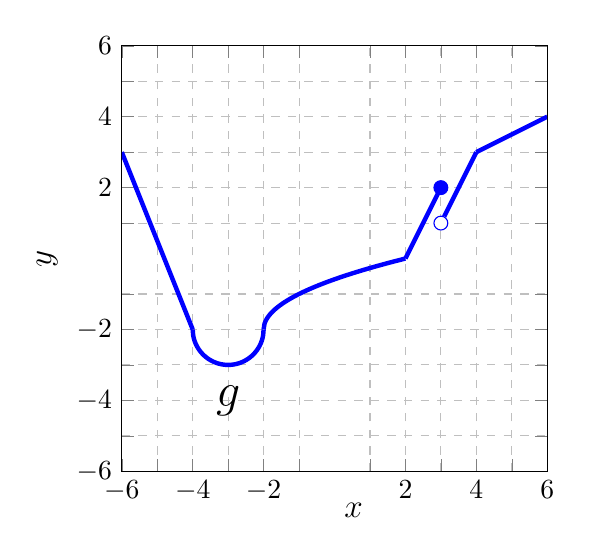
\begin{tikzpicture}[scale=1]
          \begin{axis}[
        %    axis y line = left,
        %    axis x line = bottom,
            xlabel = {\large$x$},
                            xlabel style={anchor=west},
            ylabel = {\large$y$},
                            ylabel style={anchor=south},
            xtick       = {-6,-5, -4, -3,-2,-1,1,2,3, 4, 5, 6},
            xticklabels = {$-6$, , $-4$, ,$-2$,,,$2$,, $4$, , $6$},
            ytick       = {-6,-5, -4, -3,-2,-1,1,2,3, 4, 5, 6},
            yticklabels = {$-6$, , $-4$, ,$-2$,,,$2$,, $4$, , $6$},
            samples     = 160,
            domain      = 0:3,
            restrict y to domain=-10:100,
            xmin = -6, xmax = 6,
            ymin = -6, ymax = 6,
            width=2.75in,height=2.75in,
            grid=both, grid style=dashed
          ]
          %
%          \addplot[domain=-6:-4, red, ultra thick, mark=none] {x + 9};
%          %
%          \addplot[domain=-4:-3, red, ultra thick, mark=none] {5};
%          %
%          \addplot[domain=-3:0, red, ultra thick, mark=none] {-2/3 * x + 3};
%          %
%          \addplot[domain=0:1, red, ultra thick, mark=none] {-7*x+3};
%          \addplot[domain=1:3, red, ultra thick, mark=none] {-2 - (4 - (x-1)^2)^(0.5)};
%          \addplot[domain=3:5, red, ultra thick, mark=none] {-2 - (4 - (x-5)^2)^(0.5)};
%          \addplot[domain=3:5, red, ultra thick, mark=none] {-2 - (4 - (x-5)^2)^(0.5)};
%          \addplot[domain=5:6, red, ultra thick, mark=none] {-4 + 0.5*(x-5)^2};
%          %
%          \filldraw[black] (-3,3) circle (0pt) node[] {\LARGE $f$};
          %
          %\draw[->,thick] (-0.9,1.9) -- (-0.35,1.6);
          %
          \addplot[domain=-6:-4, blue, ultra thick, mark=none] {-5/2 *x -12};
          %
          \addplot[domain=-4:-2, blue, ultra thick, mark=none] {-2 - (1 - (x+3)^2)^(1/2)};
          \addplot[domain=-2:2, blue, ultra thick, mark=none] {(x+2)^(1/2) - 2};
          %
          \addplot[domain=2:3, blue, ultra thick, mark=none] {2*x-4};
          \addplot[domain=3:4, blue, ultra thick, mark=none] {2*x-5};
          \filldraw[white] (3,1) circle (2.5pt);
          \draw[blue] (3,1) circle (2.5pt);
          \filldraw[blue] (3,2) circle (2.5pt);
          \addplot[domain=4:6, blue, ultra thick, mark=none] {0.5*x+1};
          %
          \filldraw[black] (-3,-4) circle (0pt) node[] {\LARGE $g$};
          %
          %\draw[->,thick] (0.3,-1.5) -- (-0.2,-1.3);
          %
        \end{axis}
    \end{tikzpicture}    
\end{center}
}
}
%
%\hfill
%
%\begin{minipage}[t][2.5in]{0.3\textwidth}


\newpage

\section{Draw the graph of a function satisfying each set of criteria}


    \begin{enumerate}
    \item[(a)] $f'(1)=0,f(1)=2$, $f$ is not differentiable at $x=3$, and $\ds \lim_{x\to 3^-}f(x) = -3$. \\
        \mpageT{.6}{.4}{
        \,
        }
        {
        \begin{center}
    \begin{tikzpicture}[scale=1]
          \begin{axis}[
        %    axis y line = left,
        %    axis x line = bottom,
            xlabel = {\large$x$},
                            xlabel style={anchor=west},
            ylabel = {\large$y$},
                            ylabel style={anchor=south},
            xtick       = {-6,-5, -4, -3,-2,-1,1,2,3, 4, 5, 6},
            xticklabels = {$-6$, , $-4$, ,$-2$,,,$2$,, $4$, , $6$},
            ytick       = {-6,-5, -4, -3,-2,-1,1,2,3, 4, 5, 6},
            yticklabels = {$-6$, , $-4$, ,$-2$,,,$2$,, $4$, , $6$},
            samples     = 160,
            domain      = 0:3,
            restrict y to domain=-10:100,
            xmin = -4, xmax =4 ,
            ymin = -4, ymax =4 ,
            width=2.75in,height=2.75in,
            grid=both, grid style=dashed
          ]
        \end{axis}
    \end{tikzpicture}    
\end{center}
}
\vfill
    \item[(b)] $f'(3)=-1$, but the average rate of change of $f(x)$ between $x=2$ and $x=4$ is 1. (i.e. $\ds \frac{f(4)-f(2)}{4-2}=1$)\\
        \mpageT{.6}{.4}{
        \,
        }
        {
        \begin{center}
    \begin{tikzpicture}[scale=1]
          \begin{axis}[
        %    axis y line = left,
        %    axis x line = bottom,
            xlabel = {\large$x$},
                            xlabel style={anchor=west},
            ylabel = {\large$y$},
                            ylabel style={anchor=south},
            xtick       = {-6,-5, -4, -3,-2,-1,1,2,3, 4, 5, 6},
            xticklabels = {$-6$, , $-4$, ,$-2$,,,$2$,, $4$, , $6$},
            ytick       = {-6,-5, -4, -3,-2,-1,1,2,3, 4, 5, 6},
            yticklabels = {$-6$, , $-4$, ,$-2$,,,$2$,, $4$, , $6$},
            samples     = 160,
            domain      = 0:3,
            restrict y to domain=-10:100,
            xmin = -4, xmax =4 ,
            ymin = -4, ymax =4 ,
            width=2.75in,height=2.75in,
            grid=both, grid style=dashed
          ]
        \end{axis}
    \end{tikzpicture}    
\end{center}
}
\vfill
    
    \end{enumerate}

\newpage
\section{Draw the graph of a function satisfying each set of criteria, part deaux}


    \begin{enumerate}
        \mpageT{.6}{.4}{
        \item[(a)] Sketch a graph of a function with the following properties:\\ $f(1)=1,f'(1)=1,f(5)=-1,f'(5)=-1$.\\
        }
        {
        \begin{center}
    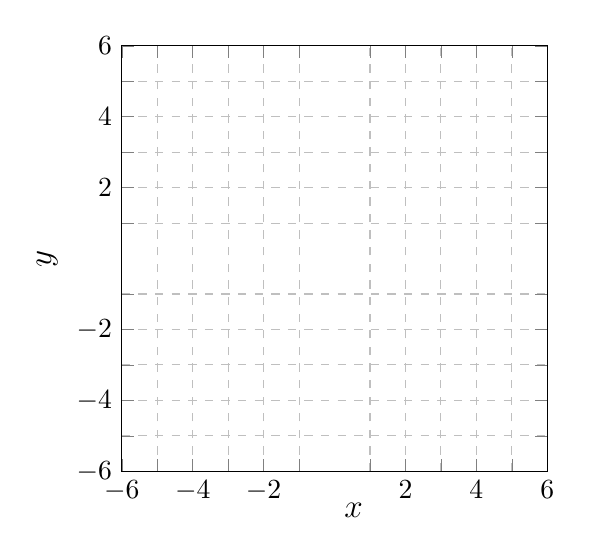
\begin{tikzpicture}[scale=1]
          \begin{axis}[
        %    axis y line = left,
        %    axis x line = bottom,
            xlabel = {\large$x$},
                            xlabel style={anchor=west},
            ylabel = {\large$y$},
                            ylabel style={anchor=south},
            xtick       = {-6,-5, -4, -3,-2,-1,1,2,3, 4, 5, 6},
            xticklabels = {$-6$, , $-4$, ,$-2$,,,$2$,, $4$, , $6$},
            ytick       = {-6,-5, -4, -3,-2,-1,1,2,3, 4, 5, 6},
            yticklabels = {$-6$, , $-4$, ,$-2$,,,$2$,, $4$, , $6$},
            samples     = 160,
            domain      = 0:3,
            restrict y to domain=-10:100,
            xmin = -6, xmax =6,
            ymin = -6, ymax =6 ,
            width=2.75in,height=2.75in,
            grid=both, grid style=dashed
          ]
        \end{axis}
    \end{tikzpicture}    
\end{center}
}

 \mpageT{.6}{.4}{
       \item[(b)] Sketch a graph of a function with the following properties:\\ $f(1)=1,f'(1)=\text{DNE}, f(3)=\text{DNE},f(5)=1,f'(5)=1$.
        }
        {
        \begin{center}
    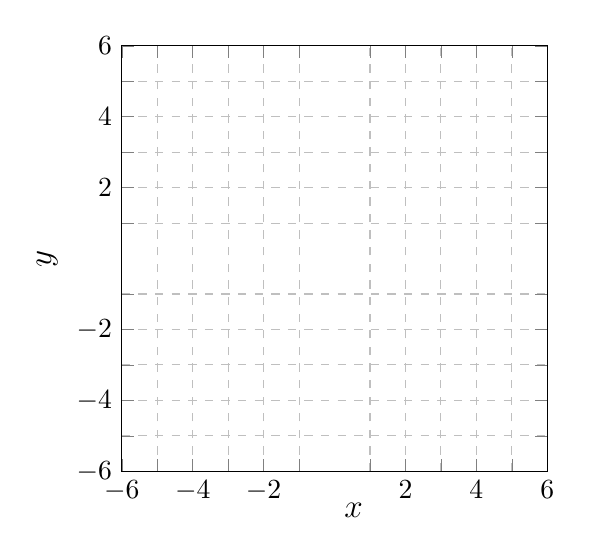
\begin{tikzpicture}[scale=1]
          \begin{axis}[
        %    axis y line = left,
        %    axis x line = bottom,
            xlabel = {\large$x$},
                            xlabel style={anchor=west},
            ylabel = {\large$y$},
                            ylabel style={anchor=south},
            xtick       = {-6,-5, -4, -3,-2,-1,1,2,3, 4, 5, 6},
            xticklabels = {$-6$, , $-4$, ,$-2$,,,$2$,, $4$, , $6$},
            ytick       = {-6,-5, -4, -3,-2,-1,1,2,3, 4, 5, 6},
            yticklabels = {$-6$, , $-4$, ,$-2$,,,$2$,, $4$, , $6$},
            samples     = 160,
            domain      = 0:3,
            restrict y to domain=-10:100,
            xmin = -6, xmax =6,
            ymin = -6, ymax =6 ,
            width=2.75in,height=2.75in,
            grid=both, grid style=dashed
          ]
        \end{axis}
    \end{tikzpicture}    
\end{center}
}

\end{enumerate}
\newpage
\section{Creating the derivative function}
In this problem, you will estimate the derivative of the function $f(x)=x^2$ at various points, then use those estimates to guess at the general formula of the ``derivative machine" function that generates them.

\begin{enumerate}
    \item Consider the function $f(x) = x^2$.
    \begin{enumerate}
        \item We want to compute the derivative \[f'(a) = \lim_{h\to 0}\frac{f(a+h) - f(a)}{h}\]
        for various values of $a$. Feel free to use any techniques we've seen to compute these limits. Some things you can try are:
        \begin{itemize}
            \item compute the quantity for very small values of $h$,
            \item use algebraic manipulations to simplify, or
            \item find a line with slope equal to the result of the limit and estimate that.
        \end{itemize}
        Record your answers here, and show your work on a separate page.
        \[
            \arraycolsep=20pt
            \begin{array}{c|ccccc}
                a & -2 & -1 & 0 & 1 & 2 \\ \hline
                f'(a) & 
            \end{array}
        \]
\vspace{0.5cm}
        \item Now, plot the values you found as points $\big(a,f'(a)\big)$ below.
        \begin{center}
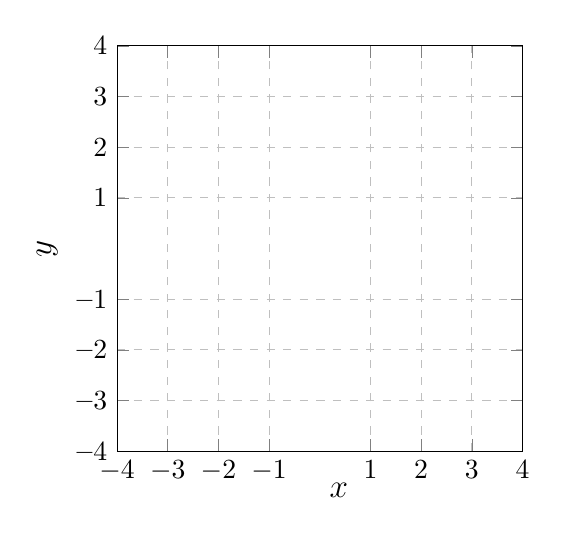
\begin{tikzpicture}[]
      \begin{axis}[
    %    axis y line = left,
    %    axis x line = bottom,
        xlabel = {\large$x$},
                        xlabel style={anchor=west},
        ylabel = {\large$y$},
                        ylabel style={anchor=south},
        xtick       = {-4,-3,-2,-1,1,2,3,4},
        xticklabels = {$-4$,$-3$,$-2$,$-1$,$1$,$2$,$3$,$4$},
        ytick       = {-4,-3,-2,-1,1,2,3,4},
        yticklabels = {\textbf{--}$4$,\textbf{--}$3$,\textbf{--}$2$,\textbf{--}$1$,$1$,$2$,$3$,$4$},
        samples     = 160,
        domain      = 0:3,
        restrict y to domain=-10:100,
        xmin = -4, xmax = 4,
        ymin = -4, ymax = 4,
        width=2.65in,height=2.65in,
        grid=both, grid style=dashed
      ]
    \end{axis}
\end{tikzpicture}
\end{center}
\item Based on this data, what equation do you think describes the function which takes a number $a$ and outputs $f'(a)$?
\end{enumerate}
\end{enumerate}
\newpage

\section{Suppose you had an arbitrary function $f$}
\begin{enumerate}
    \item[(a)] Write an expression to find the \textbf{slope of the secant line} of $f$ between $x = 2$ and $x = 4$
        \vfill
    \item[(b)] Write an expression to find the \textbf{average rate of change} of $f$ between $x = a$ and $x = a+h$
        \vfill
    \item[(c)] Building off of part (b), write an expression (involving a limit) to find the instantaneous rate of change of $f$ at $x = 3$. What does the limit represent?
        \vfill
    \item[(d)] Explain what the following expression represents:
    \[\frac{f(x) - f(1)}{x - 1}\]
        \vfill
    \item[(e)] Explain what the following expression represents:
    \[\lim_{x \to 1}\frac{f(x) - f(1)}{x - 1}\]
        \vfill

    
    \end{enumerate}



%}





\end{document}